
\subsection{Expected Cross-Correlation}\label{sec:syn_ecc}

\subsubsection{A maximum likelihood estimation formulation for the CC metric}
The squared Normalized Cross Correlation metric (which we will refer to simply as ``Cross Correlation'' metric) can be obtained as the cost function associated to a maximum likelihood estimation problem derived from the following observation model. We assume that, if the two images $I, J$ are correctly aligned, then the voxel intensities of all corresponding local windows are linearly correlated (either positively, or negatively). To make this statement more precise, let's focus on one single window $\mathcal{W}_{v}\subset\Omega_{R}$ centered at one specific voxel $v$. Denote by $X = (I(w_{1}), I(w_{2}), ..., I(w_{n})), w_{i}\in\mathcal{W}_{v}$ the vector whose entries are the intensity values of image $I$ at the voxels that compose window $\mathcal{W}_{v}$. Similarly, denote by $Y = (J(w_{1}), J(w_{2}), ..., J(w_{n}))$. Then we assume that, if $I, J$ are correctly aligned, then there exists a linear relation between $X$ and $Y$:
\begin{equation}\label{eq:local_linearity_assumption}
    \begin{array}{lcl}
        Y &=& cX + \epsilon, c \neq 0, \epsilon \sim N(0, \sigma^{2}\mathbb{I})
    \end{array}
\end{equation}
where $c\in\mathbb{R}$ is a scalar, which may be positive or negative, indicating whether $X,Y$ are positively or negatively correlated, and $\epsilon$ is a random vector accounting for white (i.e. independent) noise. Each entry of $\epsilon$ corresponds to the noise distortion occurred at one specific voxel, and we further assume that they are normally distributed with a common standard deviation $\sigma$. The technical assumption $c \neq 0$ is used here to avoid the degenerate case where at least one of the images is constant in $\mathcal{W}_{v}$, which will be treated as a special case. The Normality assumption is made to make the problem more tractable; the analysis under more general or realistic noise models is beyond the scope of this work.\\

From eq. \eqref{eq:local_linearity_assumption} we can see that $X = \frac{1}{c}(Y - \epsilon)$, and:
\begin{equation}\label{eq:dot_products}
    \begin{array}{lclcl}
        X^{T}Y &=& \frac{1}{c}(Y-\epsilon)^{T}Y &=& \frac{1}{c}Y^{T}Y - \frac{1}{c}Y^{T}\epsilon\\[2mm]
        X^{T}Y &=& X^{T}(cX + \epsilon) &=& cX^{T}X + X^{T}\epsilon
    \end{array}
\end{equation}
and equivalently, by dividing by a multiple of each squared norm:
\begin{equation}\label{eq:normalized_dot_products}
    \begin{array}{lclcl}
        \frac{X^{T}Y}{\frac{1}{c}||Y||^{2}} &=& 1 - \frac{Y^{T}\epsilon}{||Y||^{2}}\\[2mm]
        \frac{X^{T}Y}{c||X||^{2}} &=& 1 + \frac{X^{T}\epsilon}{c||X||^{2}}
    \end{array}
\end{equation}
therefore, by multiplying both equations we obtain:
\begin{equation}\label{eq:squared_dot_product}
    \begin{array}{lcl}
        \frac{\left(X^{T}Y\right)^{2}}{||X||^{2}||Y||^{2}} &=& \left(1 - \frac{Y^{T}\epsilon}{||Y||^{2}}\right)\left(1 + \frac{X^{T}\epsilon}{c||X||^{2}}\right)
    \end{array}
\end{equation}
and equivalently:
\begin{equation}\label{eq:squared_dot_product}
    \begin{array}{lcl}
        1-\frac{\left(X^{T}Y\right)^{2}}{||X||^{2}||Y||^{2}} &=& \left(\frac{Y^{T}}{||Y||^{2}} - \frac{X^{T}}{c||X||^{2}}\right)\epsilon + \frac{\epsilon^{T}Y X^{T}\epsilon}{c||Y||^{2}||X||^{2}}.
    \end{array}
\end{equation}
We can identify in the left-hand side of eq. \eqref{eq:squared_dot_product} the squared normalized cross correlation metric $CC(X, Y) = \frac{\left(X^{T}Y\right)^{2}}{||X||^{2}||Y||^{2}}$. It turns out that maximization of $CC(X, Y)$ implies the minimization of the negative log-likelihood from eq. \eqref{eq:local_linearity_assumption}, which can be proven as follows. Assume that $CC(X, Y)$ is relatively close to one (by Jensen's inequality, it is always less than or equal to one):
\begin{equation}\label{eq:hypothesis_tau}
    \frac{\left(X^{T}Y\right)^{2}}{||X||^{2}||Y||^{2}} \geq 1-\tau^{2}, \tau\in[0,1].
\end{equation}
Let's choose the correlation factor $c = \frac{X^{T}Y}{||X||^{2}}$ (the maximum likelihood estimator for $c$). The negative log-likelihood from eq. \eqref{eq:local_linearity_assumption} is of the form $K_{0} + \frac{1}{2\sigma^{2}}||Y - cX||^{2}$, where $K_{0}$ is the logarithm of the normalization constant from the multi-variate Normal distribution, and
\begin{equation}\label{eq:residual}
    ||Y - cX||^{2} = ||Y - \frac{X^{T}Y}{||X||^{2}}X||^{2} = ||Y||^{2} - 2\frac{(X^{T}Y)^{2}}{||X||^{2}} + \frac{(X^{T}Y)^{2}}{||X||^{2}}
\end{equation}
but by hypothesis (eq. \eqref{eq:hypothesis_tau}),
\begin{equation}
    ||Y||^{2} \leq \frac{\left(X^{T}Y\right)^{2}}{||X||^{2}(1-\tau^{2})}
\end{equation}
which implies, from eq. \eqref{eq:residual} that
\begin{equation}
    ||Y - cX||^{2} \leq \frac{\left(X^{T}Y\right)^{2}}{||X||^{2}(1-\tau^{2})} - \frac{(X^{T}Y)^{2}}{||X||^{2}} =
    \frac{(X^{T}Y)^{2}\tau^{2}}{||X||^{2}(1-\tau^{2})}
\end{equation}
which approaches zero when $\tau$ goes to zero (i.e., when the cross-correlation approaches 1). In summary, maximization of the CC metric is equivalent to a maximum-likelihood estimation according to the model given by eq. \eqref{eq:local_linearity_assumption}. In the registration framework, the parameters with respect to which this maximization is performed are precisely the parameters defining the transformation aligning images $I, J$. Another way of looking at this process is to imagine that the transformation attempts to make the local relationship between intensities of $X,Y$ as linear as possible.\\

\subsubsection{Local cross correlation with globally estimated transfer}

In the mono-modal case, the cross correlation metric has been proven to be very robust, which means that eq. \eqref{eq:local_linearity_assumption} is an adequate model for image registration. However, in the multi-modal case, the relationship between intensities of $I$ and $J$ may not be accurately described by a local linear model. We aim to extend this model to account for global non-linear relationships between intensities of $I$ and $J$.\\

Let's assume that there exists a map $F$ that assigns intensities from the modality of image $I$ to each intensity from the modality of image $J$, such that the local relationship between intensities of both modalities is approximately affine. More precisely:
\begin{equation}
    F[y] = cx + b + \epsilon.
\end{equation}
If we denote by $X = \left[x \; \mathbf{1}\right]$, where $\mathbf{1}$ is a column of the same length as $x$ with all its entries equal to $1$, then we may write
\begin{equation}
    F[y] = X\beta + \epsilon
\end{equation}
where the value of $\beta = \left(c, b\right)^{T}$ can be directly obtain by minimizing $|| F[y] - X\beta||^{2}$ with respect to $\beta$, which yields
\begin{equation}
    \widehat{\beta} = \left(X^{T}X\right)^{-1}X^{T}F[y].
\end{equation}

Therefore our observation model may be written as
\begin{equation}
    F[y] =  X\left(X^{T}X\right)^{-1}X^{T}F[y] + \epsilon.
\end{equation}
Note that, since $F$ is a function that only depends on the intensities of $y$, our objective is to assign a value $f_{i}$ to each intensity $i$ such that the residual error
\begin{equation}\label{eq:ecc_transfer_objective}
    || F[y] - X\left(X^{T}X\right)^{-1}X^{T}F[y]||^{2} = || P F[y]||^{2}
\end{equation}
is minimized, where $P = \mathbbm{I} - X\left(X^{T}X\right)^{-1}X^{T}$. The minimizer of the above expression is not unique. To see why this is a natural property of our model, assume that $F^{*}$ is an optimal transfer. then any affine transform $F = r F^{*} + s$ is also an optimal transfer because $F[y] = r F^{*}[y]+s = r(cx+b)+s = (rc)x + (b+s)$. A degenerate election would, for example, be $F^{*} = 0$.\\

To write equation \eqref{eq:ecc_transfer_objective} in terms of the vector $f$, we can group all entries $y_{i}$ of $y$ according to its value $\ell \in C$ and write the product $P F[y]$ as:
\begin{equation}
    P F[y] = \sum_{\ell \in C} f_{\ell} \sum_{i: y_{i} = \ell} P e_{i}
\end{equation}
where $e_{i}$ is the $i$-th basis vector (which means $P e_{i}$ is the $i-$th column of P). Let's denote this sum of column vectors as
\begin{equation}
    s_{\ell} =  \sum_{i: y_{i} = \ell} P e_{i}
\end{equation}
and define the matrix $S$ by concatenating all columns $s_{\ell}, \ell\in C$ together:
\begin{equation}
    S = [s_{1}, s_{2}, ..., s_{|C|}].
\end{equation}
Our objective is to minimize
\begin{equation}
    \sum_{v \in \Omega} ||S^{v} f||^{2}.
\end{equation}

Note that $S^{v}$ is a $n\times m$ matrix, where $n$ is the number of voxels contained in the local windows, and $m=|C|$ is the number of quantized intensities in $C$.
\begin{equation}
    \left(X^{T}X\right)^{-1} =
        \left(\begin{array}{cc}
            x^{T}x & x^{T}\mathbbm{1}\\
            x^{T}\mathbbm{1} & n\\
        \end{array}\right)^{-1} =
        \frac{1}{n x^{T}x - \left(x^{T}\mathbbm{1}\right)^{2}}
        \left(\begin{array}{cc}
            n & -x^{T}\mathbbm{1}\\
            -x^{T}\mathbbm{1} & x^{T}x
        \end{array}\right)
\end{equation}
\begin{equation}
    X\left(X^{T}X\right)^{-1}X^{T} =
        \frac{1}{n x^{T}x - \left(x^{T}\mathbbm{1}\right)^{2}}
        \left[x \; \mathbbm{1}\right]\left(\begin{array}{cc}
            n & -x^{T}\mathbbm{1}\\
            -x^{T}\mathbbm{1} & x^{T}x
        \end{array}\right)
        \left[\begin{array}{c}
            x^{T}\\
            \mathbbm{1}^{T}
        \end{array}\right]=
\end{equation}
\begin{equation}
        \frac{1}{n x^{T}x - \left(x^{T}\mathbbm{1}\right)^{2}}
        \left[x \; \mathbbm{1}\right]
        \left[\begin{array}{c}
            n x^{T} - x^{T}\mathbbm{1}\mathbbm{1}^{T}\\
            -x^{T}\mathbbm{1}x^{T} + x^{T}x\mathbbm{1}^{T}
        \end{array}\right]
\end{equation}
the $i-$th column of $\mathbbm{I} - X\left(X^{T}X\right)^{-1}X^{T}$ is
\begin{equation}
        e_{i} - \frac{1}{n x^{T}x - \left(x^{T}\mathbbm{1}\right)^{2}}
        \left[x \; \mathbbm{1}\right]
        \left[\begin{array}{c}
            n x_{i} - x^{T}\mathbbm{1}\\
            -x^{T}\mathbbm{1}x_{i} + x^{T}x
        \end{array}\right]=
\end{equation}
\begin{equation}
        e_{i} - \frac{1}{n x^{T}x - \left(x^{T}\mathbbm{1}\right)^{2}}
        \left[(n x_{i} - x^{T}\mathbbm{1})x + (x^{T}x - x^{T}\mathbbm{1}x_{i})\mathbbm{1}\right] =
\end{equation}
\begin{equation}
        e_{i} - \frac{n}{n x^{T}x - \left(x^{T}\mathbbm{1}\right)^{2}}
        \left[x_{i}\left(x - \bar{x}\mathbbm{1}\right) + \left(\frac{x^{T}x}{n}\mathbbm{1} - \bar{x}x\right)\right]=
        e_{i} - \frac{n}{\Delta}\left[x_{i}u + v\right]
\end{equation}
The sum $s_{\ell}$ can then be written as
\begin{equation}
        s_{\ell} = \sum_{i:y_{i}=\ell} e_{i} - \frac{n}{\Delta}\left[x_{i}u+v\right] = E_{\ell} - \frac{n\sum_{i:y_{i}=\ell}x_{i}}{\Delta}u - \frac{nk_{l}}{\Delta}v = E_{\ell} - \frac{n}{\Delta}\left(a_{\ell}u + k_{\ell}v \right).
\end{equation}
Note that $E_{\ell}^{T}E_{\ell'} = 0 \forall \ell \neq \ell'$ and  $E_{\ell}^{T}E_{\ell'} = k_{l}$ if $\ell=\ell'$, then the product of two of these vectors is
\begin{equation}
    s_{\ell}^{T}s_{\ell'} =
    \left\lbrace\begin{array}{l}
        E_{\ell}^{T}E_{\ell'} -\\
        \frac{n}{\Delta}\left[(a_{\ell'}E_{\ell} + a_{\ell}E_{\ell'})^{T}u + (k_{\ell'}E_{\ell}+k_{\ell}E_{\ell'})^{T}v\right]+\\
        \frac{n^{2}}{\Delta^{2}}\left(
            k_{\ell}k_{\ell'}||v||^{2}
            + \left(k_{\ell}a_{\ell'} + k_{\ell'}a_{\ell}\right)u^{T}v
            +a_{\ell}a_{\ell'}||u||^{2}\right)
    \end{array}\right.
\end{equation}
Now let's compute the individual terms:

\begin{equation}
    E_{\ell}^{T}u = \sum_{i:y_{i}=\ell}\left(x_{i} - \bar{x}\right) = a_{\ell} - k_{\ell}\bar{x}
\end{equation}
\begin{equation}
    E_{\ell}^{T}v = \sum_{i:y_{i}=\ell}\left(\frac{x^{T}x}{n} - \bar{x}x_{i}\right) = \frac{k_{\ell}x^{T}x}{n} - \bar{x}a_{\ell}
\end{equation}
\begin{equation}
    ||u||^{2} = \left(x - \bar{x}\mathbbm{1}\right)^{T}\left(x - \bar{x}\mathbbm{1}\right) = x^{T}x - n\bar{x}^{2}
\end{equation}
\begin{equation}
    u^{T}v = \left(x - \bar{x}\mathbbm{1}\right)^{T}\left(\frac{x^{T}x}{n}\mathbbm{1} - \bar{x}x\right) = -\frac{\bar{x}\Delta}{n}
\end{equation}

\begin{equation}
    ||v||^{2} = \left(\frac{x^{T}x}{n}\mathbbm{1} - \bar{x}x\right)^{T}\left(\frac{x^{T}x}{n}\mathbbm{1} - \bar{x}x\right) = \frac{(x^{T}x)^{2}}{n} - (x^{T}x)\bar{x}^{2}
\end{equation}
And  the product of two columns is
\begin{equation}
    s_{\ell}^{T}s_{\ell'} =
    \left\lbrace\begin{array}{l}
        E_{\ell}^{T}E_{\ell'} -\\
        \frac{2}{\Delta}\left[k_{\ell}k_{\ell'}x^{T}x -(k_{\ell}a_{\ell'} +k_{\ell'}a_{\ell})x^{T}\mathbbm{1}+ n a_{\ell}a_{\ell'}\right]+\\
        \frac{1}{\Delta}\left[k_{\ell}k_{\ell'} x^{T}x - (k_{\ell}a_{\ell'}+k_{\ell'}a_{\ell})x^{T}\mathbbm{1} + n a_{\ell}a_{\ell'}\right]
    \end{array}\right.
\end{equation}
or:
\begin{equation}
    s_{\ell}^{T}s_{\ell'} = E_{\ell}^{T}E_{\ell'} - \frac{1}{\Delta}\left[k_{\ell}k_{\ell'}x^{T}x -(k_{\ell}a_{\ell'} +k_{\ell'}a_{\ell})x^{T}\mathbbm{1}+ n a_{\ell}a_{\ell'}\right]
\end{equation}

In summary, for each window we need to compute $x^{T}x, x^{T}\mathbbm{1}$ and $k_{\ell}, a_{\ell} \forall \ell\in C$.



\begin{figure}[t!]
\centering
    \subfloat[]{\label{fig:T1T2_affine_fit_map}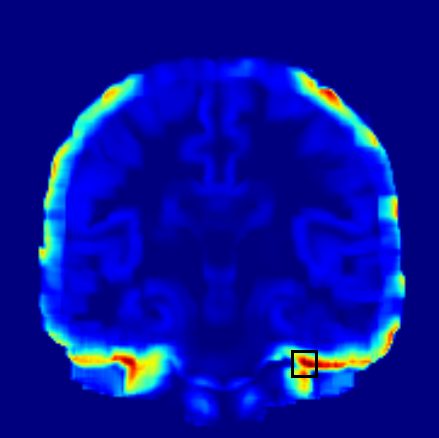
\includegraphics[width=0.33\linewidth]{./images/residuals_input_sample1.png}}
    \subfloat[]{\label{fig:T1T2_affine_fit_scatter1}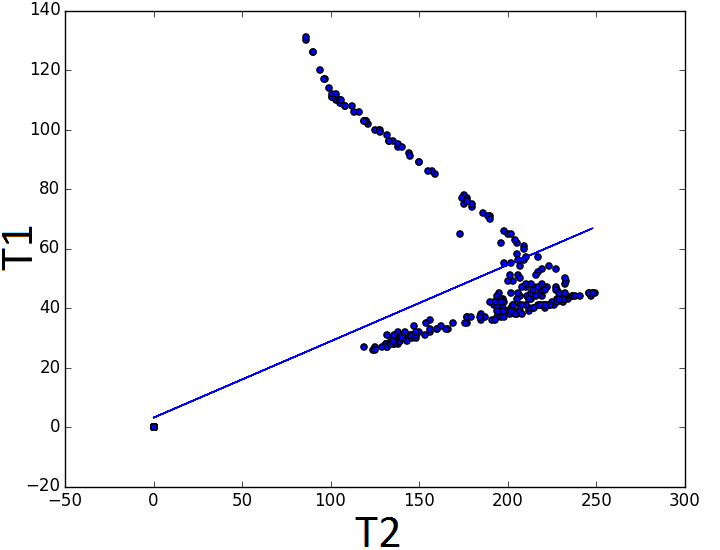
\includegraphics[width=0.33\linewidth]{./images/t1_aafo_t2_sample1.png}}
    \subfloat[]{\label{fig:T1T2_affine_fit_scatter2}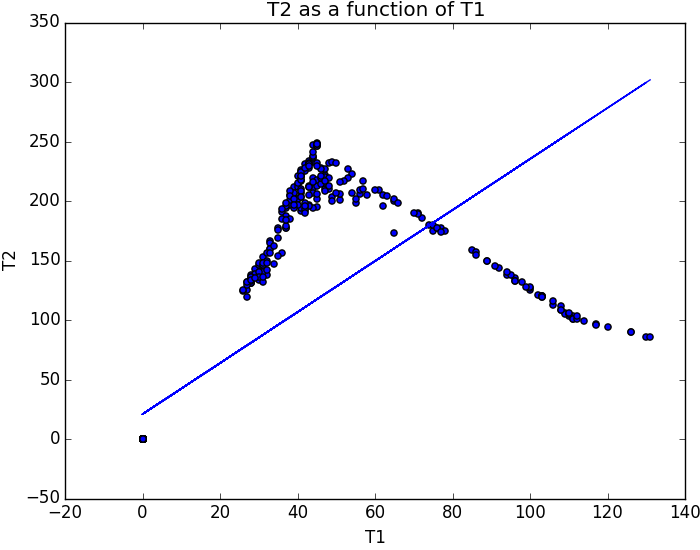
\includegraphics[width=0.33\linewidth]{./images/t2_aafo_t1_sample1.png}}\\
    \subfloat[]{\label{fig:T1FT2_affine_fit_map}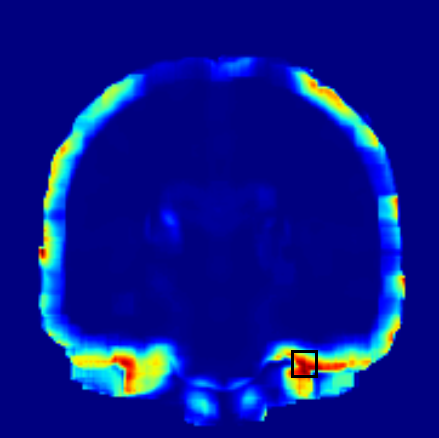
\includegraphics[width=0.33\linewidth]{./images/residuals_t1_sample1.png}}
    \subfloat[]{\label{fig:T1FT2_affine_fit_scatter1}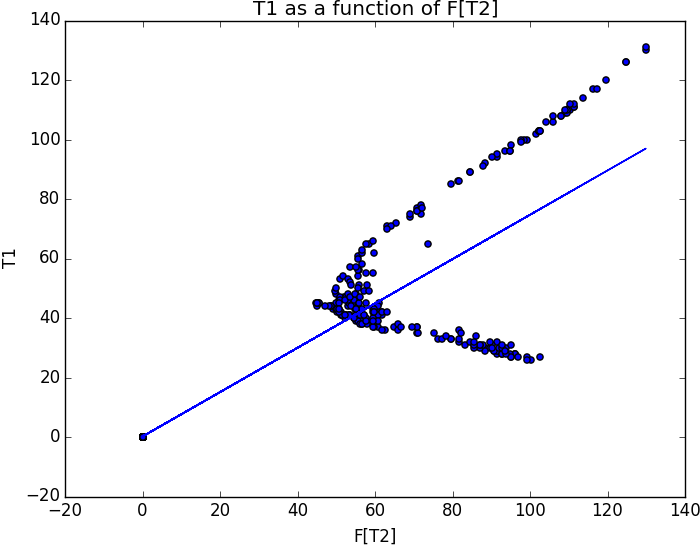
\includegraphics[width=0.33\linewidth]{./images/t1_aafo_Ft2_sample1.png}}
    \subfloat[]{\label{fig:T1FT2_affine_fit_scatter2}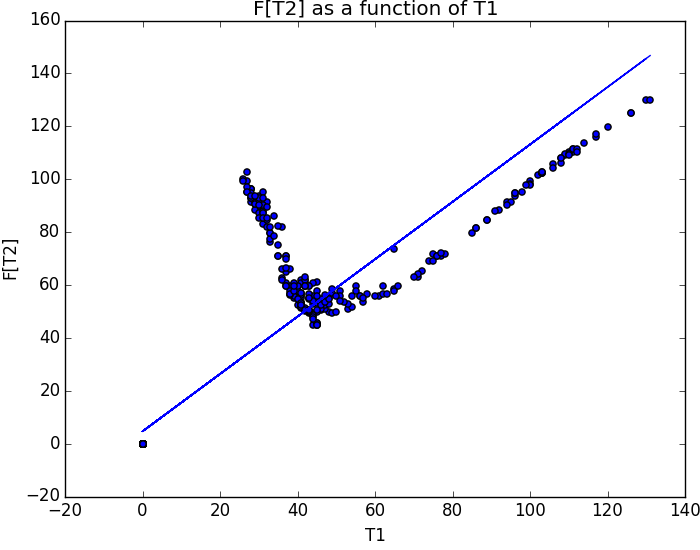
\includegraphics[width=0.33\linewidth]{./images/Ft2_aafo_t1_sample1.png}}\\
    \subfloat[]{\label{fig:FT1T2_affine_fit_map}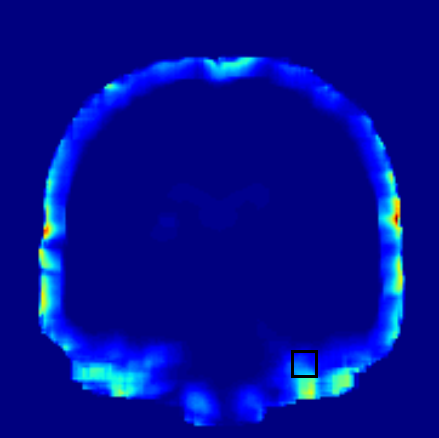
\includegraphics[width=0.33\linewidth]{./images/residuals_t2_sample1.png}}
    \subfloat[]{\label{fig:FT1T2_affine_fit_scatter1}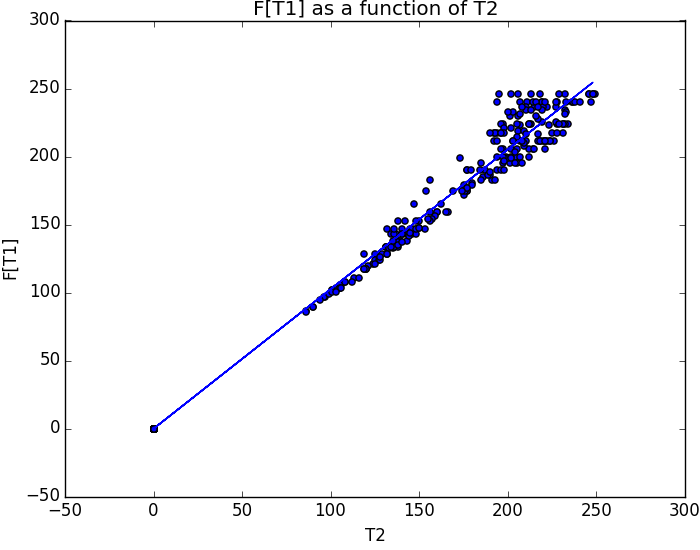
\includegraphics[width=0.33\linewidth]{./images/Ft1_aafo_t2_sample1.png}}
    \subfloat[]{\label{fig:FT1T2_affine_fit_scatter2}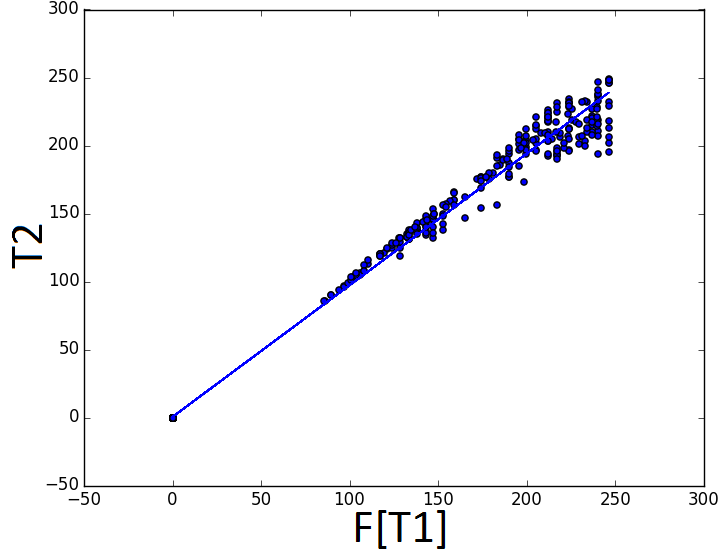
\includegraphics[width=0.33\linewidth]{./images/t2_aafo_Ft1_sample1.png}}\\
    \caption{Affine residuals.}
\label{fig:transfers}
\end{figure}


\begin{figure}[t!]
\centering
    \subfloat[]{\label{fig:T1T2_affine_fit_scatter1}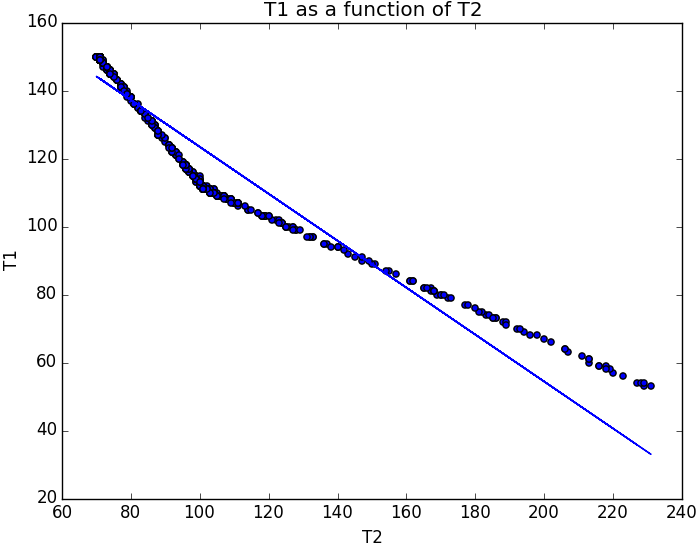
\includegraphics[width=0.2\linewidth]{./images/t1_aafo_t2_sample2.png}}
    \subfloat[]{\label{fig:T1T2_affine_fit_scatter2}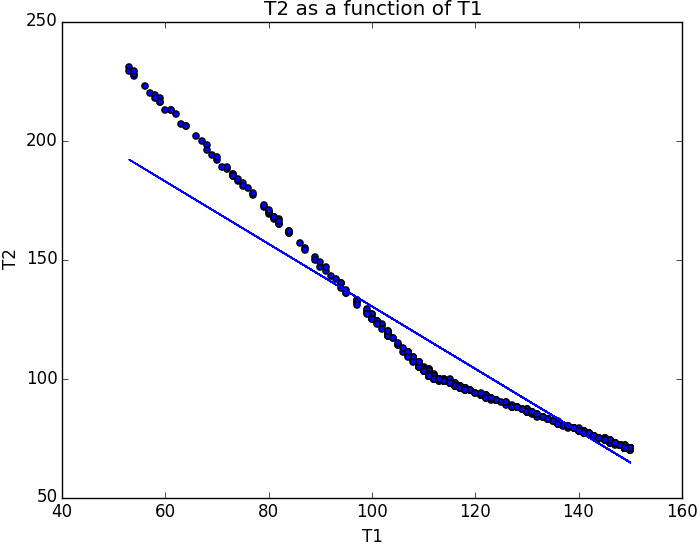
\includegraphics[width=0.2\linewidth]{./images/t2_aafo_t1_sample2.png}}
    \subfloat[]{\label{fig:T1T2_affine_fit_map}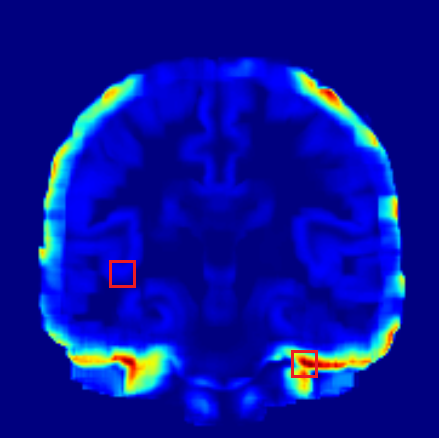
\includegraphics[width=0.2\linewidth]{./images/residuals_input.png}}
    \subfloat[]{\label{fig:T1T2_affine_fit_scatter1}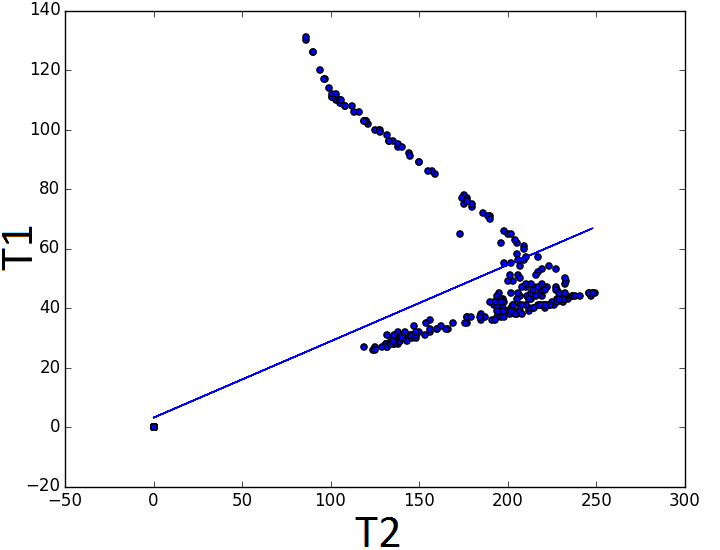
\includegraphics[width=0.2\linewidth]{./images/t1_aafo_t2_sample1.png}}
    \subfloat[]{\label{fig:T1T2_affine_fit_scatter2}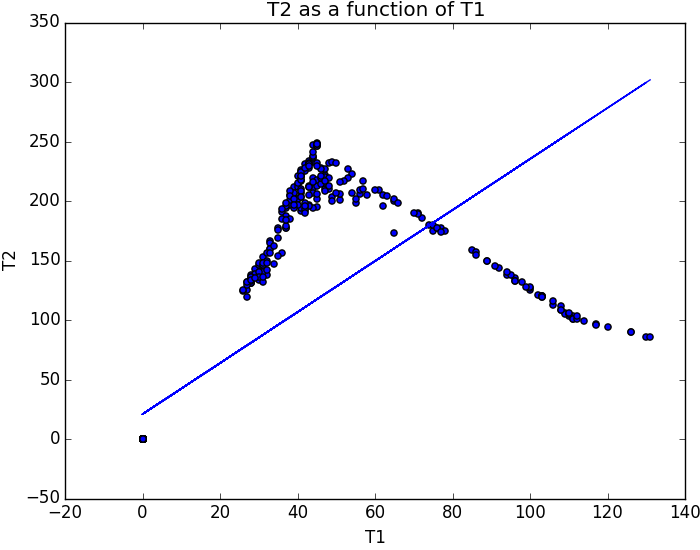
\includegraphics[width=0.2\linewidth]{./images/t2_aafo_t1_sample1.png}}\\
    \subfloat[]{\label{fig:T1FT2_affine_fit_scatter1}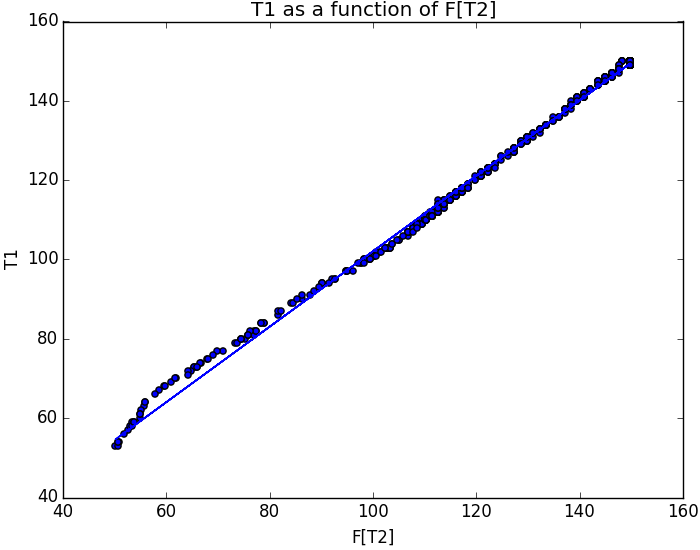
\includegraphics[width=0.2\linewidth]{./images/t1_aafo_Ft2_sample2.png}}
    \subfloat[]{\label{fig:T1FT2_affine_fit_scatter2}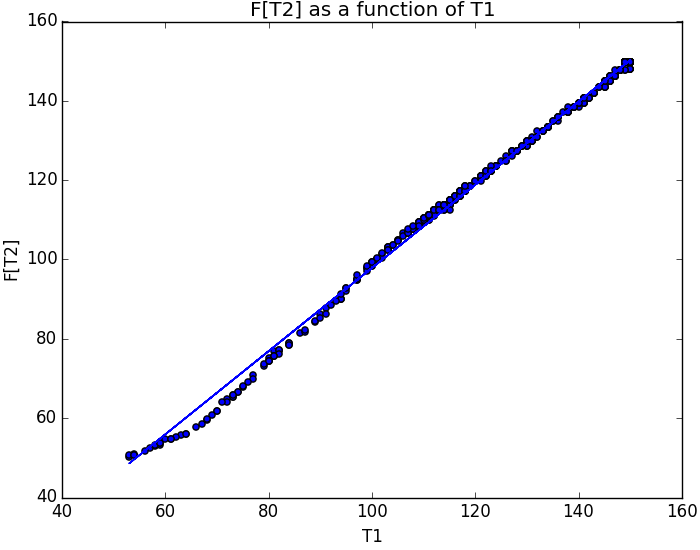
\includegraphics[width=0.2\linewidth]{./images/Ft2_aafo_t1_sample2.png}}
    \subfloat[]{\label{fig:T1FT2_affine_fit_map}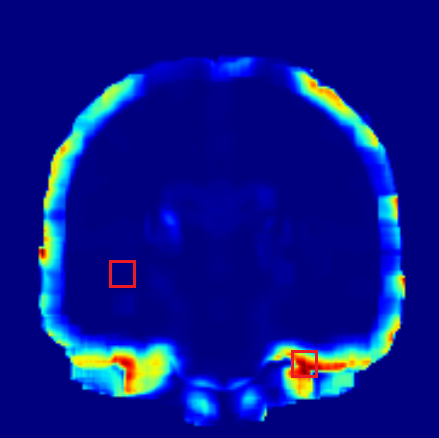
\includegraphics[width=0.2\linewidth]{./images/residuals_t1.png}}
    \subfloat[]{\label{fig:T1FT2_affine_fit_scatter1}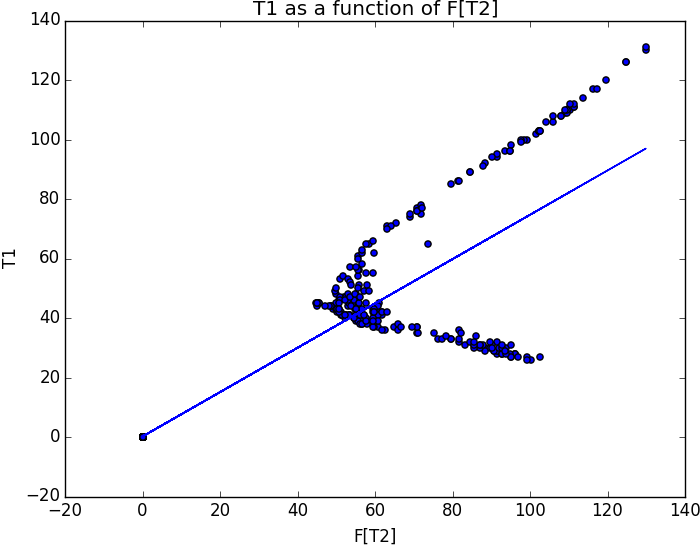
\includegraphics[width=0.2\linewidth]{./images/t1_aafo_Ft2_sample1.png}}
    \subfloat[]{\label{fig:T1FT2_affine_fit_scatter2}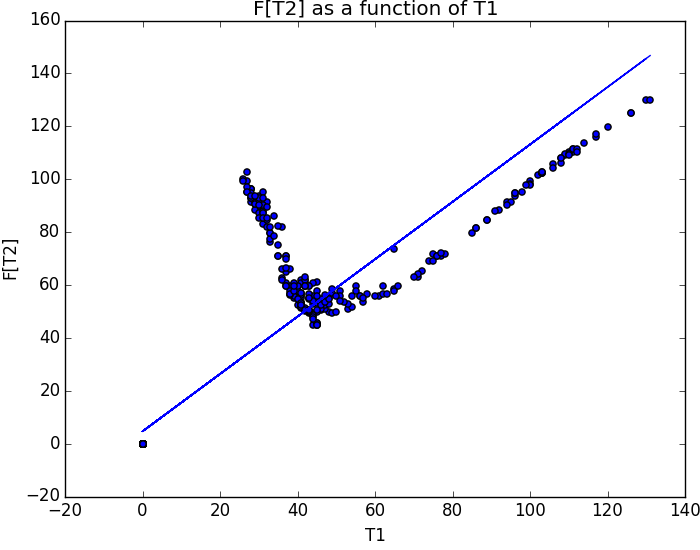
\includegraphics[width=0.2\linewidth]{./images/Ft2_aafo_t1_sample1.png}}\\
    \subfloat[]{\label{fig:FT1T2_affine_fit_scatter1}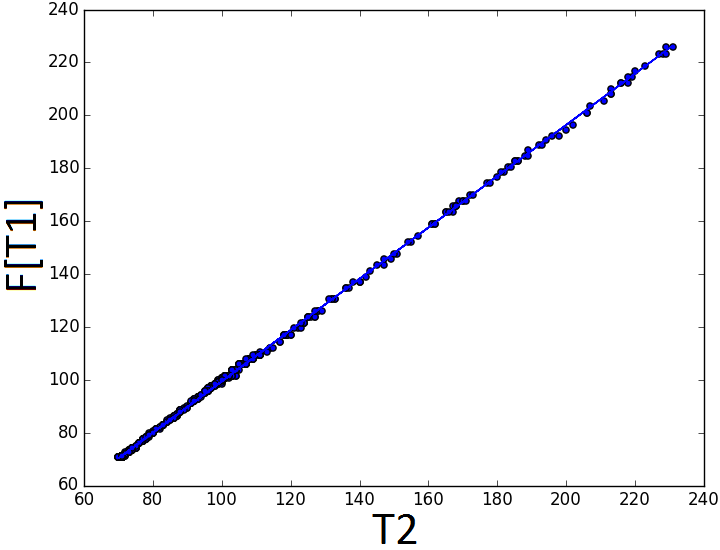
\includegraphics[width=0.2\linewidth]{./images/Ft1_aafo_t2_sample2.png}}
    \subfloat[]{\label{fig:FT1T2_affine_fit_scatter2}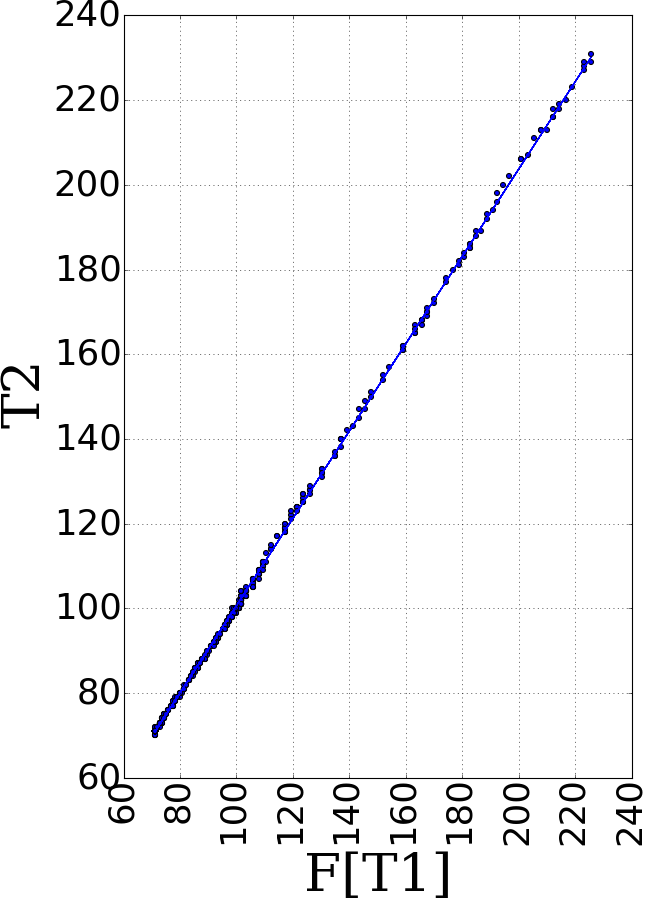
\includegraphics[width=0.2\linewidth]{./images/t2_aafo_Ft1_sample2.png}}
    \subfloat[]{\label{fig:FT1T2_affine_fit_map}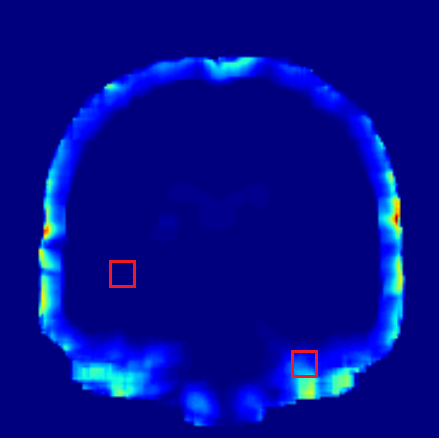
\includegraphics[width=0.2\linewidth]{./images/residuals_t2.png}}
    \subfloat[]{\label{fig:FT1T2_affine_fit_scatter1}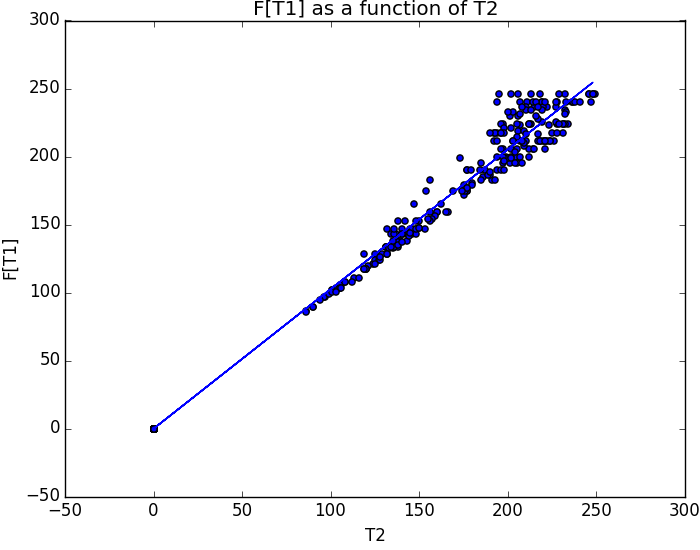
\includegraphics[width=0.2\linewidth]{./images/Ft1_aafo_t2_sample1.png}}
    \subfloat[]{\label{fig:FT1T2_affine_fit_scatter2}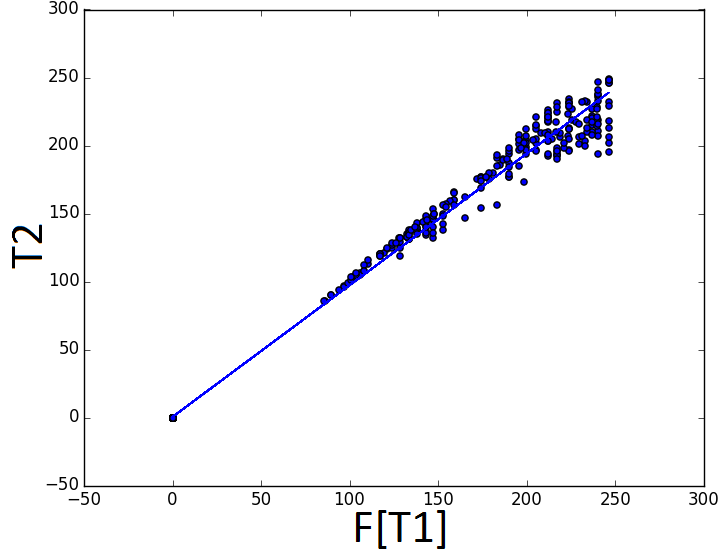
\includegraphics[width=0.2\linewidth]{./images/t2_aafo_Ft1_sample1.png}}\\
    \caption{Residual error of best line describing the relationship between intensities of both modalities under perfect alignment (using the Brainweb synthetic template). a)-e): original T1-T2 images. Right scatter plots correspond to the right ROI in the middle panel. Left scatter plots correspond to the left ROI. f)-j): T1-F[T2] (where F is the mean transfer function mapping T2 intensities to T1 intensities). k)-o): F[T1]-T2 (where F is the mean transfer function mapping T2 intensities to T1 intensities) }
\label{fig:transfers}
\end{figure}



The main drawback of using a point-wise metric like SSD, the EM metric previously described, or Mutual Information, is that they are unable to capture important features from the voxels' neighborhood like gradients and texture. Being point-wise, any permutation of the voxels' positions results in exactly the same measured similarity (provided the same permutation is applied to both, the moving and fixed images). This makes point-wise metrics more susceptible to noise and image artifacts such as the bias field in MRI. By considering small windows $W_{y}$ around each voxel $y\in\Omega_{R}$, the normalized Cross Correlation metric (CC), takes advantage of more complex local information, resulting in a more robust metric:
\begin{equation}
    CC(y;\tilde{I}, \tilde{J}) = \frac{\left[\sum_{z\in W_{y}} \left(\tilde{I}(z) - \mu_{y}\right)\left(\tilde{J}(z) - \nu_{y}\right)\right]^{2}}
    {\left[\sum_{z \in W_{y}}\left(\tilde{I}(z) - \mu_{y}\right)^{2}\right] \left[\sum_{z \in W_{y}}\left(\tilde{J}(z) - \nu_{y}\right)^{2}\right]}
\end{equation}
where
\begin{equation}
    \begin{array}{lll}
        \mu_{y} &=& \frac{1}{|W_{y}|}\sum_{z \in W_{y}}\tilde{I}(z)\\
        \nu_{y} &=& \frac{1}{|W_{y}|}\sum_{z \in W_{y}}\tilde{J}(z)\\
    \end{array}.
\end{equation}

The EM formulation belongs to the class of multi-modal image registration methods that reduce the multi-modal problem to a mono-modal one \citep{Sotiras2013}. One of the advantages of this class of methods is that it is relatively easy to extend other mono-modal metrics to the multi-modal case using the same ideas. In particular, we can extend the CC metric for multi-modal images by defining the {\it Expected Cross Correlation} metric as:
\begin{equation}\label{eq:ecc_metric}
    ECC(y;\tilde{I}, \tilde{J}) = CC(y; \overline{Y}, \tilde{I}) + CC(y; \overline{Z}, \tilde{J})
\end{equation}

The first term measures the similarity between $\overline{Y}$ and $\tilde{I}$ (corresponding to a similarity measure in the modality of $I$), while the second term measures the
similarity between $\overline{Z}$ and $\tilde{J}$ (corresponding to a similarity measure in the modality of $J$). The resulting algorithm (see Appendix \ref{ap:Algorithms}, alg. \ref{alg:SyNECC}) is, therefore, a combination of the Greedy-SyN algorithm (\ref{alg:Greedy_SyN}) and the SyN-EM algorithm (see Appendix \ref{ap:CC_gradient} for details on
computing the gradients).


\subsection{Experiments}
Validation is one of the most challenging aspects of developing image registration algorithms. In order to rigorously evaluate the performance of non-linear
image registration algorithms, we would require a ground-truth consisting of true correspondences between voxels of realistic pairs of images. Since such a ground-truth data are not currently available, researchers resort to surrogates that indirectly measure the quality of their algorithms. For brain MRI registration, for instance, one of the most accepted surrogate measures, is based on the overlap of localized anatomical areas of registered images: ideally, corresponding anatomical areas of perfectly registered images should perfectly overlap. Even a perfect registration algorithm is unlikely to achieve such an ambitious goal, though, since anatomical areas are usually defined manually by an expert, which is by no means a perfect process and the annotations may vary even between different experts. Despite this limitation, it has been shown that among the alternative surrogate measures usually employed, overlap scores of localized anatomical areas is the one that better distinguish reasonable from inaccurate registrations \citep{Rohlfing2012} and it has been employed in the most rigorous evaluations of registration algorithms \citep{Klein2009, Klein2010, Rohlfing2012}. In our experiments, we employ the publicly available Internet Brain Segmentation Repository (IBSR) database consisting of 18 manually annotated T1 brain MRI volumes. Our algorithms are publicly available from the Dipy non-linear registration module \citep{Garyfallidis2014}.\\

The methods under evaluation in this section are: 1) SyN with the Normalized Cross Correlation metric \citep{Avants2008, Avants2011}, denoted ``SyN-CC'', 2) SyN with the Mutual Information metric \citep{Mattes2003, Avants2011}, denoted ``SyN-MI'', available in the ANTs software package, 3) the SyN-EM algorithm (see Appendix \ref{ap:Algorithms}, alg. \ref{alg:SyNEM}) proposed in section \ref{sec:syn_em}, and 4) the SyN-ECC algorithm (see Appendix \ref{ap:Algorithms}, alg. \ref{alg:SyNECC}) proposed in section \ref{sec:syn_ecc}. 